\documentclass{article}
\usepackage{multicol}
\usepackage{amsfonts}
\usepackage{amsmath}
\usepackage{amssymb}
\usepackage{graphicx}
\usepackage{xcolor}
\usepackage{enumitem}
\usepackage[font=small, labelfont=bf, justification=centering]{caption}
\usepackage[colorlinks=true, linkcolor=black, urlcolor=red, citecolor=black]{hyperref}
\usepackage[a4paper, margin=1in]{geometry}

\begin{document}
  {\centering \textbf{Problema 1} \par}
  Definimos a sequência \( (a_n)_n \) de forma recursiva, onde os termos iniciais são \( a_1 = 12 \) e \( a_2 = 24 \), e para \( n \geq 3 \), temos
  \[
    a_n = a_{n-2} + 14.
  \]
  \begin{enumerate}[label=(\alph*)]
    \item O número 2023 aparece na sequência?
    \item Mostre que não existem quadrados perfeitos nessa sequência.
  \end{enumerate}

  \medskip

  {\centering \textbf{Resposta} \par}

  \textbf{(a)} Não, já que não existem números ímpares nesta sequência. Basta perceber que $a_1$ e $a_2$ são pares, logo $a_{n-2}$ nunca será ímpar.

  \textbf{(b)} Digamos que existem quadrados perfeitos na sequência, logo, podemos dizer que $x^2 = 12 + 14y$ ou $x^2 = 24 + 14y$ $\Rightarrow$ $y = \frac{x^2 - 12}{14} $ ou 
  $y = \frac{x^2 - 24}{14}$ $\Rightarrow$ $x^2 \equiv 12 \pmod{14}$. A tabela abaixo mostra que isso é um absurdo, já que $\forall x \in \{k \in \mathbb{Z}^+ \mid k < 14 \},
  \quad x \not\equiv 12 \pmod{14}$
  \begin{multicols}{2}
    \begin{enumerate}
      \item $x^2 = 1 \Rightarrow 1 \equiv 1 \pmod{14}$
      \item $x^2 = 4 \Rightarrow 4 \equiv 4 \pmod{14}$
      \item $x^2 = 9 \Rightarrow 9 \equiv 9 \pmod{14}$
      \item $x^2 = 16 \Rightarrow 16 \equiv 2 \pmod{14}$
      \item $x^2 = 25 \Rightarrow 25 \equiv 11 \pmod{14}$
      \item $x^2 = 36 \Rightarrow 36 \equiv 8 \pmod{14}$
      \item $x^2 = 49 \Rightarrow 49 \equiv 7 \pmod{14}$
      \item $x^2 = 64 \Rightarrow 64 \equiv 8 \pmod{14}$
      \item $x^2 = 81 \Rightarrow 81 \equiv 11 \pmod{14}$
      \item $x^2 = 100 \Rightarrow 100 \equiv 2 \pmod{14}$
      \item $x^2 = 121 \Rightarrow 121 \equiv 9 \pmod{14}$
      \item $x^2 = 144 \Rightarrow 144 \equiv 4 \pmod{14}$
      \item $x^2 = 169 \Rightarrow 169 \equiv 1 \pmod{14}$
    \end{enumerate}
  \end{multicols}

  \noindent\rule{\linewidth}{0.4pt}

  {\centering \textbf{Problema 2} \par}
  Sejam \( a, b, c \) números reais tais que \( a^n + b^n = c^n \) para três valores inteiros positivos consecutivos de \( n \). Prove que \( abc = 0 \).

  \medskip

  {\centering \textbf{Resposta} \par}

  Dado:
  \[
    a^n + b^n = c^n, a^{n+1} + b^{n+1} = c^{n+1}, a^{n+2} + b^{n+2} = c^{n+2}
  \]
  Pode-se afirmar que
  \[
    c = \frac{a^{n+1} + b^{n+1}}{a^n + b^n} \quad \text{e} \quad c = \frac{a^{n+2} + b^{n+2}}{a^{n+1} + b^{n+1}}
  \]
  Isso resulta em:
  \[
    (a^{n+1} + b^{n+1})^2 = (a^{n+2} + b^{n+2})(a^n + b^n)
  \]
  Logo,
  \[
    2ab = a^2 + b^2 \quad \Rightarrow \quad a^2 - 2ab -b^2 = 0 \quad \Rightarrow \quad (a-b)^2 = 0 \quad \Rightarrow \quad a = b
  \]
  Para finalizar, veja abaixo que  pelo menos um dentre $a,b,c$ é 0
  \[
    c^n = 2a^n \quad \Rightarrow \ \quad c = \frac{2a^{n+1}}{2a^n} \quad \Rightarrow \quad c = a \quad \Rightarrow \quad a^n = 2a^n \quad \Rightarrow \quad a^n = 0
  \]

  \noindent\rule{\linewidth}{0.4pt}

  {\centering \textbf{Problema 3} \par}
  Em um triângulo acutângulo \( ABC \), sejam \( D \) e \( E \) os pés das alturas relativas aos vértices \( A \) e \( B \), respectivamente, e seja \( M \) o
  ponto médio de \( AC \). O círculo que passa por \( D \) e é tangente à reta \( BE \) em \( B \) intersecta a reta \( BM \) em um ponto \( F \), com \( F \ne B \). Mostre que
  \( FM \) é bissetriz de \( \angle AFD \).

  \medskip

  {\centering \textbf{Resposta} \par}

  \begin{figure}[h]
    \centering
    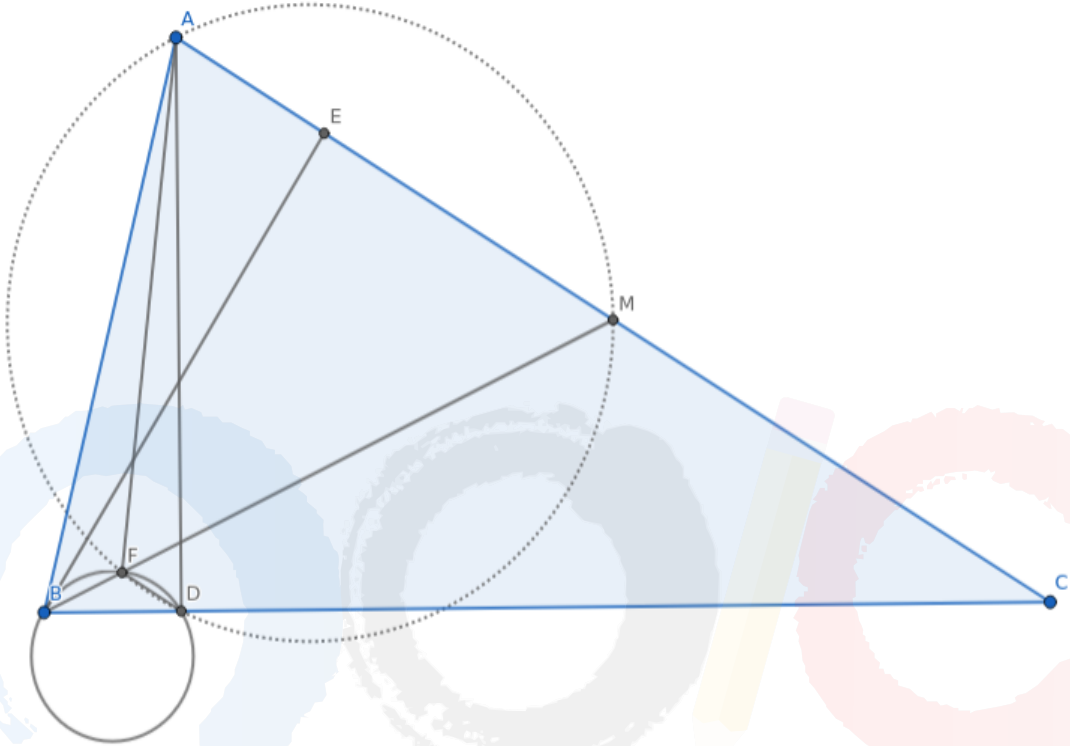
\includegraphics[width=0.5\textwidth]{first.png}
    \caption{Uma ilustração da solução do terceiro problema. \href{https://noic.com.br/wp-content/uploads/2023/11/Solucoes_da_TM2_Nivel_A.pdf}{Fonte}}
  \end{figure}

  Dado:
  \[
    \angle DAC = \angle EBC = 90^\circ - \angle C \quad \text{e} \quad \angle EBC = \angle EBM + \angle MBC.
  \]

  Pelo \textit{teorema do segmento alterno}:
  \[
    \angle EBM = \angle FDB \Rightarrow \angle MFD = \angle FDB + \angle FBD = 90^\circ - \angle C,
  \]
  
  portanto, \( AFDM \) é um quadrilátero cíclico.

  Além disso:
  \[
    \angle DFM = \angle DAM \quad \text{e} \quad \angle AFM = \angle ADM.
  \]

  Como \( MD \) é mediana de \( \triangle ADC \), tem-se:
  \[
    MA = MD = MC \Rightarrow \triangle ADC \text{ é isósceles} \Rightarrow \angle MAD = \angle ADM.
  \]

  \noindent\rule{\linewidth}{0.4pt}

  {\centering \textbf{Problema 4} \par}
  Determine todos os inteiros positivos \( n \) para os quais existe um tabuleiro \( n \times n \), onde podemos escrever \( n \) vezes cada um dos números de
  \( 1 \) a \( n \) (um número em cada casa), de modo que as \( n \) somas dos números em cada linha deixem \( n \) restos distintos na divisão por \( n \), e as \( n \) somas dos
  números em cada coluna deixem \( n \) restos distintos na divisão por \( n \).

  \medskip

  {\centering \textbf{Resposta} \par }

  Deve-se perceber que para todo $n$ ímpar, a configuração abaixo satisfaz o enunciado,
  mas nenhum $n$ par satisfaz tal.

  \begin{figure}[h]
    \centering
    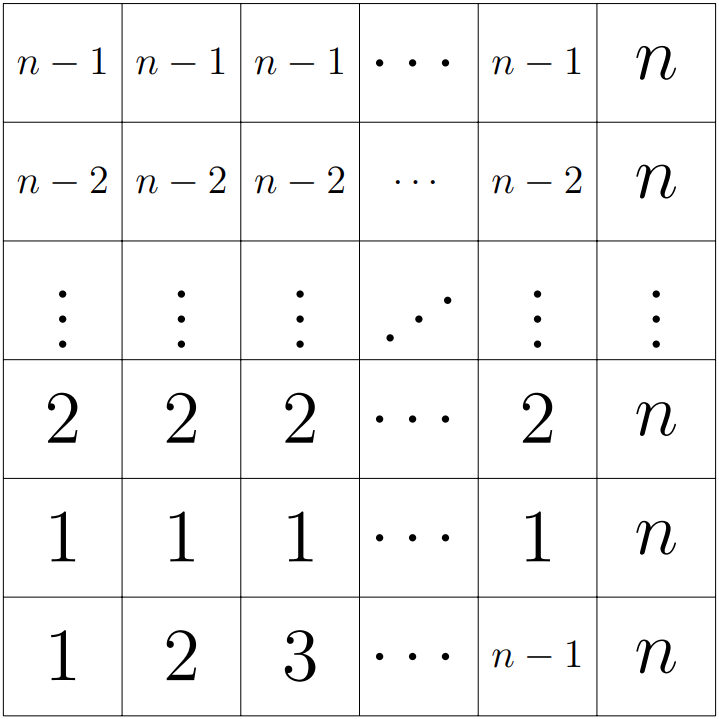
\includegraphics[width=0.3\textwidth]{second.png}
    \caption{Uma ilustração da solução do quarto problema. \href{https://noic.com.br/wp-content/uploads/2025/03/Solucoes_do_TM2_2024_Nivel_A.pdf}{Fonte}}
  \end{figure}
  
  Para provar que todas as linhas têm somas diferentes $\pmod{n}$, deve-se perceber que,
  para quaisquer duas linhas distintas entre si e distintas entre a última linha, é
  possível achar este absurdo:
  \[
    x(n-1) + n \equiv y(n-1) + n \pmod{n} \Rightarrow x \equiv y \pmod{n}
  \]
  Já para qualquer linha distinta da última linha, é possível encontrar este outro 
  absurdo, já que n é um número ímpar e $\frac{n}{2}$ não é um inteiro:
  \[
    x(n-1) + n \equiv \frac{n(n+1)}{2} \pmod{n} \Rightarrow x \equiv \frac{n}{2} \pmod{n}
  \]
  Já para $n$ igual a um número par, a soma de todos os números no tabuleiro é igual
  a $\frac{n^2(n+1)}{2}$ e a soma de todos os números $\pmod{n}$ é igual a 
  $0 + 1 + 2 + ... + (n - 1) = \frac{n(n-1)}{2}$, logo:
  \[
    \frac{n^2(n+1)}{2} \equiv \frac{n(n-1)}{2} \pmod{n} \Rightarrow \frac{n(n^2+1)}{2} \equiv 0 \pmod{n}
  \]
  $n$ é par, logo $\frac{n}{2} \in \mathbb{Z}$. Logo, pode-se encontrar o absurdo
  abaixo, que anula a existência de um número $n$ par:
  \[
    \frac{n(n^2 + 1)}{2} \equiv \frac{n}{2} \equiv 0 \pmod{n}
  \]
\end{document}

